\documentclass[border=5mm,tikz]{standalone}
\usepackage{tikz}
\begin{document}

  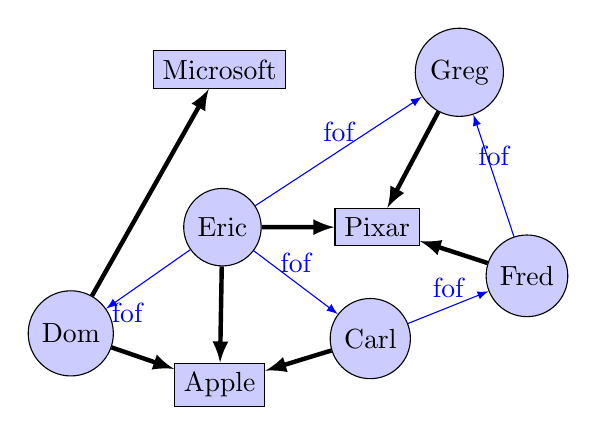
\begin{tikzpicture}
    \foreach \ang/\lab/\User in {0/C/Carl,72/E/Eric,144/D/Dom} {
      \node[circle,fill=blue!20,draw] (\lab) at ({\ang+17}:2){\User};
    }
    %\path[-latex,blue] (A) edge [above] node [blue] {fof} (B);
   % \path[-latex,blue] (A) edge [above] node [blue] {fof} (C);
    %\path[-latex,blue] (B) edge [above] node [blue] {fof} (D);
    \path[-latex,blue] (E) edge [near end, below] node [blue] {fof} (D);
    \path[-latex,blue] (E) edge [above] node [blue] {fof} (C);
    \node[circle,fill=blue!20,draw] (F) at (19.5:4.14){Fred};
    \node[circle,fill=blue!20,draw] (G) at (52.5:5){Greg};
    \path[-latex,blue] (C) edge [above] node [blue] {fof} (F);
    \path[-latex,blue] (F) edge [above] node [blue] {fof} (G);
    \path[-latex,blue] (E) edge [above] node [blue] {fof} (G);
    
    \node[rectangle,fill=blue!20,draw] (2) at (0,0) {Apple};
    \node[rectangle,fill=blue!20,draw] (1) at (0,4) {Microsoft};
    \node[rectangle,fill=blue!20,draw] (3) at (2,2) {Pixar};
    
       % \draw[-latex,ultra thick] (A) --(1);
       % \draw[-latex,ultra thick] (B) --(1);
        \draw[-latex,ultra thick] (D) --(1);
        
              \draw[-latex,ultra thick] (D) --(2);
              \draw[-latex,ultra thick] (C) --(2);
              \draw[-latex,ultra thick] (E) --(2);

   \draw[-latex,ultra thick] (E) --(3);
   \draw[-latex,ultra thick] (F) --(3);
   \draw[-latex,ultra thick] (G) --(3);
  \end{tikzpicture}

\end{document}